% !TEX root = hw3-answers.tex
\chead{\textbf{Exercises week 3}}

\begin{document}
\flushleft\textbf{Topic: Structural Causal Models}


\section{Nobel Prizes and Chocolate Consumption}
 (2+2 points)
 \begin{enumerate}
   \item 
     Write a program in R or Python\footnote{We recommend using R, since this is likely the more suitable programming language for the project later in the course. As an introduction, you could take a look at https://cran.r-project.org/doc/manuals/r-release/R-intro.pdf or any of the many tutorials in the internet.} for the structural causal model which is described by the equation
\begin{equation*}
  N \leftarrow \gamma + \delta C,
  \label{eq:chocolate_causes_nobel}
\end{equation*}
(treating $C$ as an exogenous input, and $N$ as endogenous)
analogous to the program in Figure 4 of the lecture notes.
In your program, simulate from the model in the observational setting, after the hard intervention
do$(C = c)$, and after the hard intervention do$(N = n)$.
As your answer, copy-paste your code and the output of the program.
   \item Now consider the more realistic structural causal model with structural equations:
     \begin{align*}
       C & \leftarrow \alpha + \beta W \\
       N & \leftarrow \gamma + \delta W,
       \label{eq:more_realistic_model}
     \end{align*}
     in which the wealth $W$ of a country is a cause of both the chocolate consumption and the number of nobel prizes.
     Here, $W$ is treated as an exogenous input variable, while $C$ and $N$ are treated as endogenous variables.
     This corresponds to equations (3) and (4) in the lecture notes. 
     Consider the three hard interventions do$(C = c)$, do$(N = n)$, and do$(W = w)$. For each of these, state which variables remain the same and which may change due to the intervention (comparing with the unintervened ``observational'' model). In how far does your answer correspond to or disagree with the intuitive causal effects between the three variables?
   \end{enumerate}

\begin{gradedsolution}
  \begin{enumerate}
    \item This is our code:
      \begin{figure}[H]
	\centering
	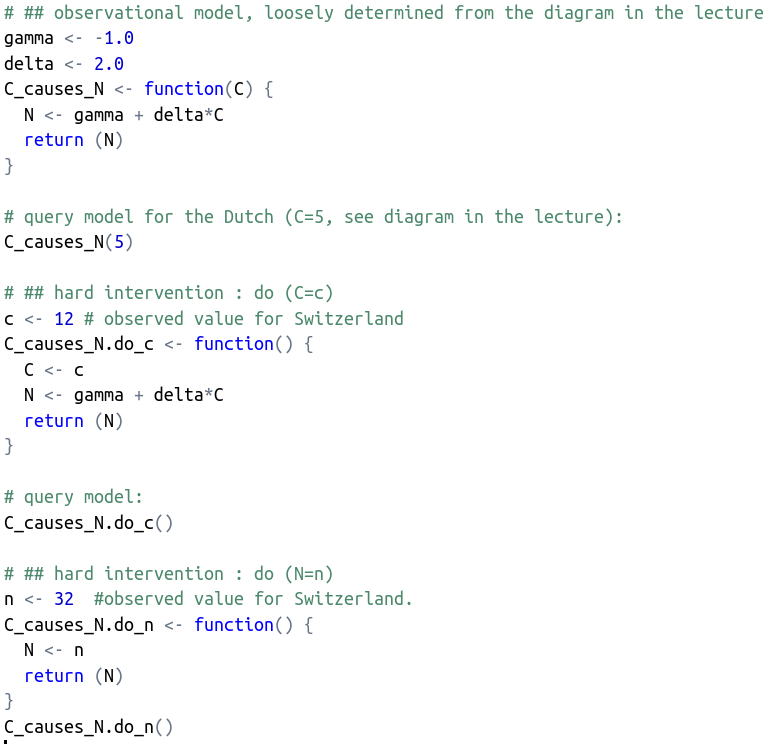
\includegraphics[width=0.8\textwidth]{r_code}
      \end{figure}
    This is the output of the code:
    \begin{figure}[H]
\centering
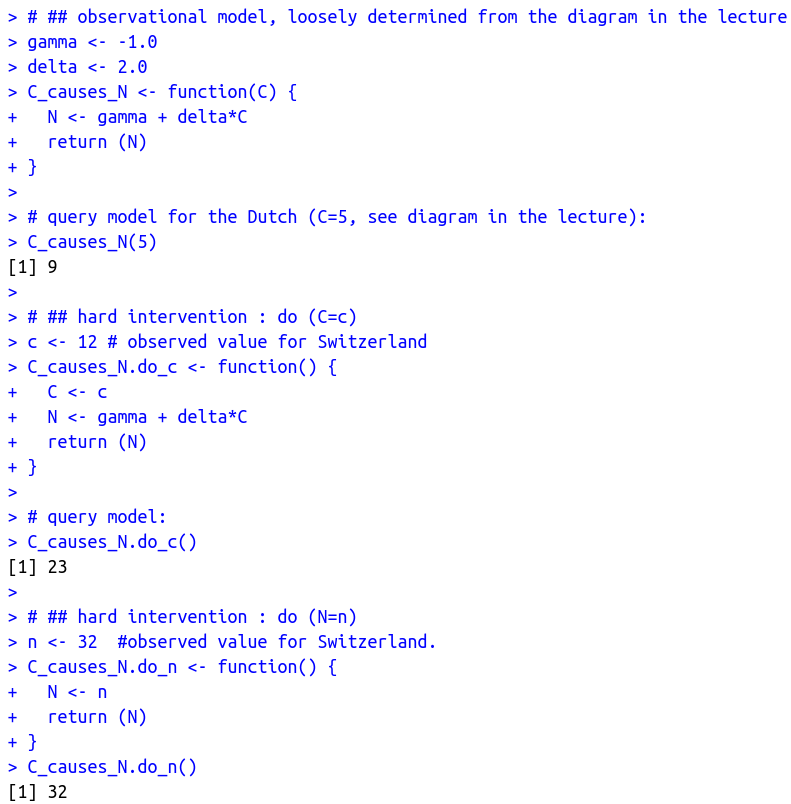
\includegraphics[width=0.8\textwidth]{r_output}
    \end{figure}
  \item A hard intervention do$(W = w)$ may change all three variables, whereas a hard intervention on chocolate consumption or nobel prices does not change any of the other variables.
    This corresponds to our intuitions on the causal effects:
    Increasing the wealth of a country may lead to more money that can be put both in chocolate and research, leading to more chocolate consumption and nobel prices.
    However, forcing people to eat more chocolate will neither change the wealth, nor the number of nobel prices, if our intuition is correct that chocolate does not contain brain enhancing chemicals (which aren't outweighed by the harms of too much chocolate consumption).
    For a hard intervention on nobel prices, it is less clear whether the model corresponds to our intuitions: it may be that a large number of nobel prices increases the attractiveness of a country for researchers, thus leading to more research and thus potentially more wealth due to industry applications. In any case, we do not expect an effect on chocolate consumption, though.
    \end{enumerate}
\end{gradedsolution}





\section{Half-adder}
(4+4 points)
\begin{figure}[h]
  \centering
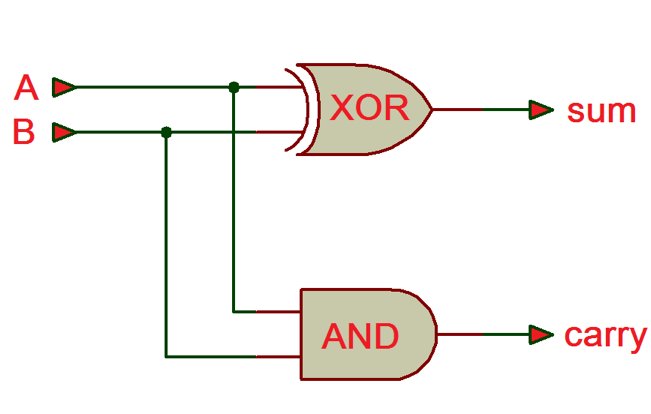
\includegraphics[width=0.6\textwidth]{half-adder-ckt}
  \caption{The half-adder is used in computers to add two bits (binary digits), with their sum represented in binary notation.
  Thus, $0 + 0 = 0$, $0 + 1 = 1$, $1 + 0 = 1$ and $1 + 1 = 10$.
  The half-adder achieves this by first computing the right-most digit, which is called the \emph{sum}, by taking the binary XOR of the two input bits. 
  Additionally, the \emph{carry} is calculated since it can happen that one digit is not enough for the result, meaning we get an additional $1$ if both A and B are $1$.
  Several half-adders can be concatenated in sequence to obtain a full-adder that can sum two natural numbers that consist of multiple bits in binary notation.
%  Then, the final result is simply the concatenation of the carry with the sum.
%  Note that this concatenation is not anymore part of the depicted model.
}
\label{fig:half-adder}
\end{figure}
Look at Figure \ref{fig:half-adder}, which specifies a so-called \emph{half-adder}.

\textbf{(a)} Assume that $A, B$ are binary exogenous \emph{input}-variables (in particular, they do not come equipped with a distribution). 
Use the symbol $S$ for the sum, and $C$ for the carry.

Do the following exercises:
\begin{enumerate}
  \item  Formally specify a structural causal model $\mathcal{M} = \left\langle \boldsymbol{\mathcal{X}}, \boldsymbol{\mathcal{Y}}, \boldsymbol{\mathcal{Z}}, P, \boldsymbol{f}\right\rangle$ for the half-adder.
  \item Determine a solution function $g: \boldsymbol{\mathcal{X}} \times \boldsymbol{\mathcal{Z}} \to \boldsymbol{\mathcal{Y}}$. Show in this specific case that it is unique (see Definition 5.7.1), without referring to exercise 3.
  \item For each combination of inputs $A$ and $B$, determine the sum and the carry.
  \item Model interventions: a hard intervention on the input A, a hard intervention on the sum S, and a soft intervention on the causal mechanism (e.g., replacing the XOR gate by an OR gate).
    What are the consequences? 
%  \item Reason about counterfactuals: if we do not observe the input, but we observe $S=1$.
%    What would the output have been, had we swapped one of the input bits?
  \end{enumerate} 

  \textbf{(b)} Now, assume that $A$ and $B$ are instead binary exogenous \emph{random} variables, i.e., they are equipped with a probability distribution.
  We assume them to be independent uniformly Bernoulli distributed.

  Do the following exercises:
  \begin{enumerate}
    \item Specify a structural causal model $\mathcal{M}'$ for this new situation.
    \item Determine the observational distributional law of the random variable $(S, C)$ with values in $\{0, 1\}^2$. 
      What is the measure-theoretic name of the operation you just performed?
    \item Perform a hard intervention on the sum $S$, forcing it to be $1$.
      Determine the corresponding interventional distribution of $(S, C)$.
    \item Instead, perform a hard intervention on the input $A$, forcing it to be $0$.
      Determine the corresponding interventional distribution of $(S, C)$.
    \end{enumerate}
\begin{gradedsolution}
  \textbf{(a)}
  \begin{enumerate}
    \item $\boldsymbol{\mathcal{X}} = \{0, 1\}^{2}$, $\boldsymbol{\mathcal{Y}} = \{0,1\}^{2}$, $\boldsymbol{\mathcal{Z}} = \{*\}$, the set with only one point. Furthermore, $P = \delta_*$, the Dirac delta distribution, is the unique distribution on $\boldsymbol{\mathcal{Z}}$. 
      Finally, $\boldsymbol{f}: \boldsymbol{\mathcal{X}} \times \boldsymbol{\mathcal{Y}} \times \boldsymbol{\mathcal{Z}} = \{0,1\}^{4} \to \{0,1\}^{2} = \boldsymbol{\mathcal{Y}}$\footnote{We use, as in other exercises as well, the convention $U \times \{*\} = U$, even though, technically, this is not an equality but only an isomorphism.} is given by
      \begin{equation}
	f \begin{pmatrix} a \\ b \\ s \\ c \end{pmatrix} = \begin{pmatrix} a \oplus b \\ a \wedge b\end{pmatrix}.
	\label{eq:causal_mechanism_half_adder}
      \end{equation}
    \item Assume we had a solution $\boldsymbol{g}: \boldsymbol{\mathcal{X}} \times \boldsymbol{\mathcal{Z}} = \{0,1\}^2 \to \{0,1\}^2 = \boldsymbol{\mathcal{Y}}$.
      By definition of a solution function, this would mean that we have for all $a, b \in \{0,1\}$ the following string of equalities:
      \begin{equation}
	\begin{pmatrix} g_S \begin{pmatrix} a \\ b\end{pmatrix} \\ g_C \begin{pmatrix} a \\ b \end{pmatrix}\end{pmatrix}
	= \boldsymbol{g} \begin{pmatrix} a \\ b\end{pmatrix} 
	= f \begin{pmatrix} a \\ b \\ \boldsymbol{g} \begin{pmatrix} a \\ b\end{pmatrix}\end{pmatrix}
	= \begin{pmatrix} a \oplus b \\ a \wedge b\end{pmatrix},
	\label{eq:string_of_equations}
      \end{equation}
      which forces the equalities $g_S \begin{pmatrix} a \\ b\end{pmatrix} = a \oplus b$ and $g_C \begin{pmatrix} a \\ b\end{pmatrix} = a \wedge b$. 
      This shows uniqueness, and by construction, this is indeed a valid solution function.
    \item We can just plug in all combinations of input bits into our solution function in order to determine the sum and the carry. Remember that the sum is given by the upper entry, and the carry by the lower entry, of the results:
      \begin{equation}
	\boldsymbol{g} \begin{pmatrix} 0 \\ 0\end{pmatrix} = \begin{pmatrix} 0 \\ 0\end{pmatrix}, \quad 
	\boldsymbol{g}  \begin{pmatrix} 1 \\ 0\end{pmatrix} = \begin{pmatrix} 1 \\ 0\end{pmatrix}, \quad 
	\boldsymbol{g}  \begin{pmatrix} 0 \\ 1\end{pmatrix} = \begin{pmatrix} 1 \\ 0\end{pmatrix}, \quad 
	\boldsymbol{g} \begin{pmatrix} 1 \\ 1\end{pmatrix} = \begin{pmatrix} 0 \\ 1\end{pmatrix}
	\label{eq:sums_and_carries}
      \end{equation}
    \item Hard intervention on the input $A$: if we set $A = 0$, then this leaves us only with the two possibilities above in which the first input of $\boldsymbol{g}$ is $0$, and similarly for $A = 1$.
      In the same way, if we do a hard intervention on $B$, then we cut away half of the possibilities.
      Note that forcing either $A$ or $B$ to be zero automatically means that the carry is zero as well.
      For the soft intervention on the causal mechanism, replacing the XOR gate with an OR gate, we obtain the following solution function:
      \begin{equation}
	\boldsymbol{g}' \begin{pmatrix} a \\ b\end{pmatrix} = \begin{pmatrix} a \lor b \\ a \land b \end{pmatrix}.
	\label{eq:new_solution_function}
      \end{equation}
      In this case, the following are the results of applying the solution function to all input bit combinations:
      \begin{equation}
        \boldsymbol{g}' \begin{pmatrix} 0 \\ 0\end{pmatrix} = \begin{pmatrix} 0 \\ 0\end{pmatrix}, \quad 
	\boldsymbol{g}'  \begin{pmatrix} 1 \\ 0\end{pmatrix} = \begin{pmatrix} 1 \\ 0\end{pmatrix}, \quad 
	\boldsymbol{g}' \begin{pmatrix} 0 \\ 1\end{pmatrix} = \begin{pmatrix} 1 \\ 0\end{pmatrix}, \quad 
	\boldsymbol{g}' \begin{pmatrix} 1 \\ 1\end{pmatrix} = \begin{pmatrix} 1 \\ 1\end{pmatrix},
	\label{eq:adapted_concrete_solutions}
      \end{equation}
      which, as you can see, only changes the very last result.
    \end{enumerate}
    \textbf{(b)}
    \begin{enumerate}
      \item $\boldsymbol{\mathcal{X}}' = \{*\}$, $\boldsymbol{\mathcal{Y}}' = \{0,1\}^{2}$, $\boldsymbol{\mathcal{Z}}' = \{0,1\}^{2}$, $P': \mathcal{P}(\boldsymbol{\mathcal{Z}}) \to [0,1]$, $P'(U) = \frac{\# U}{4}$, $\boldsymbol{f}': \{0,1\}^{4} \to \{0,1\}^{2}$, given by 
	\begin{equation}
	  \boldsymbol{f}' \begin{pmatrix} s \\ c \\ a \\ b \end{pmatrix} = \begin{pmatrix} a \oplus b \\ a \land b \end{pmatrix}.
	  \label{eq:probabilistic_case}
	\end{equation}
      \item Let $P_{(S,C)}$ the observational distributional law of the random variable $(S,C)$. 
	Let $p_{(S,C)}$ its probability mass function. 
	Then, as can easily be checked, we obtain $p_{(S,C)}\begin{pmatrix} 0 \\ 0 \end{pmatrix} = \frac{1}{4}$, $p_{(S,C)}\begin{pmatrix} 1 \\ 0 \end{pmatrix} = \frac{1}{2}$, $p_{(S,C)}\begin{pmatrix} 0 \\ 1 \end{pmatrix} = \frac{1}{4}$, $p_{(S,C)}\begin{pmatrix} 1 \\ 1 \end{pmatrix} = 0$.
	This mass function then fully determines the probability measure $P_{(S,C)}$.
	Formally, if $\boldsymbol{g}': \boldsymbol{\mathcal{Z}} = \{0,1\}^{2} \to \{0,1\}^{2} = \boldsymbol{\mathcal{Y}}$ is a solution function of the SCM $\mathcal{M}'$, then $P_{(S,C)} = g_*P'$ is the push-forward measure of the distribution on the exogenous random variable $Z$.
      \item $P_{(S,C)}\left( \begin{pmatrix} 1 \\ 0 \end{pmatrix} \middle| \text{do}(S=1)\right) = \frac{3}{4}$, $P_{(S,C)}\left( \begin{pmatrix} 1 \\ 1 \end{pmatrix} \middle| \text{do}(S=1)\right) = \frac{1}{4}$
      \item   $P_{(S,C)}\left( \begin{pmatrix} 0 \\ 0 \end{pmatrix} \middle| \text{do}(A=0)\right) = \frac{1}{2}$,   $P_{(S,C)}\left( \begin{pmatrix} 1 \\ 0 \end{pmatrix} \middle| \text{do}(A=0)\right) = \frac{1}{2}$
      \end{enumerate}
\end{gradedsolution}

\section{Acyclic SCMs are uniquely solvable---an example}
(6 points)
Consider the following set of structural equations:
\begin{align}
  Z & = U + V \cdot X \\
  V & = 2 X \\
  U & = Y - X \\
  X & = 3 Y - 4
  \label{eq:acyclic_structural_equations}
\end{align}
where all the variables $X, Z, U, V, Y$ take values in $\mathbb{R}$.
We assume that $U,V,X,Z$ are endogenous and $Y$ is an exogenous input variable in this model.
Do the following exercises:
\begin{enumerate}
  \item Find a formal structural causal model $\mathcal{M} = \left\langle \boldsymbol{\mathcal{X}}, \boldsymbol{\mathcal{Y}}, \boldsymbol{\mathcal{Z}}, P, \boldsymbol{f}\right\rangle$ that represents the structural equations above.
  \item Let $(f_W)_{W \in \{X,Z,U,V\}}$ be the components of the causal mechanism function $\boldsymbol{f}$ you found in the exercise above.
    Show that there is a \emph{topological ordering} of the variables $\{Z,X,U,V\}$, meaning that it is possible to order them in such a way that each component $f_W$ depends only on variables that appear before $W$ in the ordering.
    Formally, this means finding a bijection $\sigma: \{X, Z, U, V\} \to \{1, 2, 3, 4\}$ such that $f_{W}$ does not depend on $W'$ if $\sigma(W) \leq \sigma(W')$. 
  \item With the help of your topological ordering, find a solution function $\boldsymbol{g}: \boldsymbol{\mathcal{X}} \times \boldsymbol{\mathcal{Z}} \to \boldsymbol{\mathcal{Y}}$ for $\mathcal{M}$:
    First, explain intuitively how one can find a solution. Then, write it down formally in the form of a function $\boldsymbol{g}$.
    Finally, formally verify that it is a solution function by showing that the structural equation $\boldsymbol{g}(\boldsymbol{x}, \boldsymbol{z}) = \boldsymbol{f}(\boldsymbol{x}, \boldsymbol{g}(\boldsymbol{x}, \boldsymbol{z}), \boldsymbol{z})$ is satisfied for all $\boldsymbol{x} \in \boldsymbol{\mathcal{X}}$ and almost all $\boldsymbol{z} \in \boldsymbol{\mathcal{Z}}$.
  \item Explain intuitively why $\boldsymbol{g}$ found above is the \emph{unique} solution function, see Definition 5.7.1. This does not need to be a formal proof.
    If you are comfortable with giving proofs, however, you can also give a proof instead of an intuitive explanation.
  \item Give an example of a structural causal model $\mathcal{M}'$ which can not be topologically ordered in this sense. 
%    In order to complicate this task, we ask you that if $f'_{j_1}$ depends on $Y'_{j_2}$ in your model, that then $f'_{j_2}$ does not depend on $Y'_{j_1}$.
  \item Does your new model have a solution function? If so, is it unique? Explain.
  \end{enumerate}
  \begin{gradedsolution}
    \begin{enumerate}
      \item $\boldsymbol{\mathcal{X}} = \mathbb{R}$, $\boldsymbol{\mathcal{Y}} = \mathbb{R}^{4}$\footnote{Sorry for the notation: this is consistent with the lecture, but of course, $\mathbf{\mathcal{X}}$ contains elements $y$ corresponding to the variable $Y$, etc.}, $\boldsymbol{\mathcal{Z}} = \{*\}$, the one-point-set, $P: \{\emptyset, \boldsymbol{\mathcal{Z}}\} \to [0,1]$ is given by $P = \delta_{*}$, the Dirac measure of the only point, and, finally, $\boldsymbol{f}: \boldsymbol{\mathcal{X}} \times \boldsymbol{\mathcal{Y}} \times \boldsymbol{\mathcal{Z}} = \mathbb{R}^{5} \to \mathbb{R}^{4} = \boldsymbol{\mathcal{Y}}$\footnote{In the identification $\boldsymbol{\mathcal{X}} \times \boldsymbol{\mathcal{Y}} \times \boldsymbol{\mathcal{Z}} = \mathbb{R}^{5}$ we use the typical convention that $U \times \{*\} = U$, even though, technically, this is only an isomorphism and not an equality} is given by:
	\begin{equation}
	  f \begin{pmatrix} y \\ x \\ u \\ v \\ z\end{pmatrix}
	  = \begin{pmatrix} 3y - 4 \\ y - x \\ 2x \\ u + v \cdot x\end{pmatrix}
	  \label{eq:functional_equation}
	\end{equation}
	which we have already conveniently ordered. 
      \item They already are topologically ordered. Formally, we have $\sigma(X) = 1$, $\sigma(U) = 2$, $\sigma(V) = 3$, and $\sigma(Z) = 4$. 
      \item Intuition: We need to find a solution function $g: \boldsymbol{\mathcal{X}} \times \boldsymbol{\mathcal{Z}} = \mathbb{R} \to \boldsymbol{\mathcal{Y}} = \mathbb{R}^{4}$ such that the equation 
	\begin{align}
	  \begin{split}
	  \begin{pmatrix} g_X(y) \\ g_U(y) \\ g_V(y) \\ g_Z(y)\end{pmatrix} & = \boldsymbol{g}(y)  = \boldsymbol{g}(\boldsymbol{x}, \boldsymbol{z}) = \boldsymbol{f}(\boldsymbol{x}, \boldsymbol{g}(\boldsymbol{x}, \boldsymbol{z}), \boldsymbol{z}) 
        \\ &	  = \boldsymbol{f}(y, \boldsymbol{g}(y))  = 
	  f \begin{pmatrix} y \\ g_X(y) \\ g_U(y) \\ g_V(y) \\ g_Z(y)\end{pmatrix} = \begin{pmatrix} 3y - 4 \\ y - g_X(y) \\ 2g_X(y) \\ g_U(y) + g_V(y) \cdot g_X(y)\end{pmatrix}
	\end{split}
	  \label{eq:eq_constraint}
	\end{align}
	holds.
	Comparing the left and the right side, we get the four equations $g_X(y) = 3y - 4$, $g_U(y) = y - g_X(y)$, $g_V(y) = 2g_X(y)$, $g_Z(y) = g_U(y) + g_V(y) \cdot g_X(y)$.
	Now, we see what the topological ordering is there for: We can solve these equations one-by-one from left to right, since the ordering then ensures that all the parts which we need for computing the next component-function of $\boldsymbol{g}$ has already been computed.
	We can also imagine the variables $Y, X, U, V, Z$ to be arranged in a graph with an arrow $W \to W'$ whenever one needs $W$ in order to determine $W'$. Then, with these equations we can ``propagate forward'' the solution along the graph.
	If we do this, we end up with the following solution function:
	\begin{equation}
	  \boldsymbol{g}(y) = \begin{pmatrix} 3y - 4 \\ -2y + 4 \\ 6y - 8 \\ 18y^{2} - 50y + 36\end{pmatrix}.
	  \label{eq:the_solution_function}
	\end{equation}
	Finally, we need to show that this satisfies the structural equation.
	This holds of course by construction, but here is the formal proof:
	\begin{align*}
	  \boldsymbol{f}(y, \boldsymbol{g}(y)) & = f 
	  \begin{pmatrix} y \\ 3y - 4 \\ -2y + 4 \\ 6y - 8 \\ 18y^{2} - 50y + 36\end{pmatrix}  
	  = \begin{pmatrix} 3y - 4 \\ y - (3y - 4) \\ 2(3y - 4) \\ -2y + 4 + (6y - 8) \cdot (3y - 4)\end{pmatrix} \\
	  & = \begin{pmatrix} 3y - 4 \\ -2y + 4 \\ 6y - 8 \\ 18y^{2} - 50y + 36 \end{pmatrix}
	  = \boldsymbol{g}(y),
	  \label{eq:verify_solution}
	\end{align*}
	which verifies the solution.
      \item In Equation \eqref{eq:eq_constraint}, we assumed that $\boldsymbol{g}$ satisfies the constraint and then ended up with four equations that forced us, one by one, to write down the solution function that we found.
	This already proves uniqueness.
      \item We set $\boldsymbol{\mathcal{X}}' = \{*\}$, $\boldsymbol{\mathcal{Y}}' = \mathbb{R}$, $\boldsymbol{\mathcal{Z}}' = \{*\}$, $P' = \delta_{*}$, and $\boldsymbol{f}': \boldsymbol{\mathcal{Y}}' \to \boldsymbol{\mathcal{Y}}'$, $\boldsymbol{f}'(y) = y$.
      \item For any $y_* \in \mathbb{R}$, the function $\boldsymbol{g}_{y_*}: \boldsymbol{\mathcal{X}} \times \boldsymbol{\mathcal{Z}} = \{*\} \to \boldsymbol{\mathcal{Y}} = \mathbb{R}$ given by $\boldsymbol{g}_{y_*}(*) = y_*$ is a solution, since $\boldsymbol{f}(\boldsymbol{g}_{y_*}(*)) = \boldsymbol{g}_{y_*}(*)$ by definition of $\boldsymbol{f}$.
	Thus, there are infinitely many solutions. 
	Intuitively, this is due to a ``cycle'' (to be defined in the lecture) in the corresponding causal graph.
      \end{enumerate}
  \end{gradedsolution}





\end{document}


\section{Acyclic SCMs are uniquely solvable}
(4 points)
\textbf{Do not hand in this exercise. 
  We might have it as a regular exercise in one of the upcoming sheets, and put it already on this sheet due to its connection to exercise 3.
Thus, if you want, you can already think about it on your own.} \\

Let $\mathcal{M} = \left\langle \boldsymbol{\mathcal{X}}, \boldsymbol{\mathcal{Y}}, \boldsymbol{\mathcal{Z}}, P, \boldsymbol{f}\right\rangle$ be a structural causal model.
We assume that it is \emph{acyclic}, which we define as follows:

Assume $\boldsymbol{\mathcal{Y}} = \prod_{j = 1}^{n} \mathcal{Y}_j$ is ordered. 
Then $\boldsymbol{f}$ consists of component-functions
\begin{equation*}
  f_j: \boldsymbol{\mathcal{X}} \times \boldsymbol{\mathcal{Y}} \times \boldsymbol{\mathcal{Z}} \to \mathcal{Y}_j.
  \label{eq:component_functions}
\end{equation*}
$\mathcal{M}$ is called acyclic (with respect to this ordering of the endogenous variables) if for all $j = 1, \dots, n$, for all $(\boldsymbol{x}, \boldsymbol{z}) \in \boldsymbol{\mathcal{X}} \times \boldsymbol{\mathcal{Z}}$ and all $(y_1, \dots, y_{j-1}) \in \prod_{i = 1}^{j-1} \mathcal{Y}_i$ the restriction
\begin{align*}
  f_j(\boldsymbol{x}, (y_1, \dots, y_{j-1}, \bullet), \boldsymbol{z}): & \prod_{i = j}^{n} \mathcal{Y}_i \to \mathcal{Y}_j, \\
  &  (y_{j}, \dots, y_n) \mapsto f_j(\boldsymbol{x}, (y_1, \dots, y_n), \boldsymbol{z})
  \label{eqn:def_acyclic}
\end{align*}
is constant, i.e. does not depend on the input $(y_{j}, \dots, y_n)$.

Show that $\mathcal{M}$ is then uniquely solvable, as defined in Definition 5.7.1 of the lecture notes.
\begin{gradedsolution}
\end{gradedsolution}
